\documentclass[journal]{IEEEtran}
\usepackage[a5paper, margin=10mm]{geometry}
\usepackage{tfrupee} % Include tfrupee package


\setlength{\headheight}{1cm} % Set the height of the header box
\setlength{\headsep}{0mm}     % Set the distance between the header box and the top of the text


\setlength{\intextsep}{10pt} % Space between text and floats

\makeindex


\usepackage{cite}
\usepackage{amsmath,amssymb,amsfonts,amsthm}
\usepackage{algorithmic}
\usepackage{graphicx}
\usepackage{textcomp}
\usepackage{xcolor}
\usepackage{txfonts}
\usepackage{listings}
\usepackage{enumitem}
\usepackage{mathtools}
\usepackage{gensymb}
\usepackage{comment}
\usepackage[breaklinks=true]{hyperref}
\usepackage{tkz-euclide} 
\usepackage{listings}
\usepackage{multicol}
\usepackage{xparse}
\usepackage{color}                                            
\usepackage{array}                  
                         
\usepackage{longtable}                                     
\usepackage{calc}                                       
       
\usepackage{multirow}                                       
\usepackage{hhline}                                           
\usepackage{ifthen}            
                                
\usepackage{lscape}
\usepackage{tabularx}
\usepackage{array}
\usepackage{float}
\usepackage{ar}
\usepackage{gvv}
\usepackage[version=4]{mhchem}



\newtheorem{theorem}{Theorem}[section]
\newtheorem{problem}{Problem}
\newtheorem{proposition}{Proposition}[section]
\newtheorem{lemma}{Lemma}[section]
\newtheorem{corollary}[theorem]{Corollary}
\newtheorem{example}{Example}[section]
\newtheorem{definition}[problem]{Definition}
\newcommand{\BEQA}{\begin{eqnarray}}
\newcommand{\EEQA}{\end{eqnarray}}

\theoremstyle{remark}

\begin{document}
\bibliographystyle{IEEEtran}
\onecolumn

\title{METALLURGY ENGINEERING (MT)}
\author{GATE 2025 \\
EE25BTECH11027-INDHIRESH S}
\maketitle

\renewcommand{\thefigure}{\theenumi}
\renewcommand{\thetable}{\theenumi}

\section*{General Aptitude}
\subsection*{Q.1 - Q.5 Carry ONE mark Each}
\begin{enumerate}
\item Despite his initial hesitation, Rehman's \underline{\hspace{2cm}} to contribute to the success of the project never wavered. \hfill{\brak{\text{GATE MT 2025}}}\\
Select the most appropriate option to complete the above sentence.
\begin{multicols}{4}
\begin{enumerate}
\item ambivalence
\item satisfaction
\item resolve
\item revolve
\end{enumerate}
\end{multicols}

\item Bird : Nest :: Bee : \underline{\hspace{2cm}} \hfill{\brak{\text{GATE MT 2025}}} \\
Select the correct option to complete the analogy.
\begin{multicols}{4}
\begin{enumerate}
\item Kennel
\item Hammock
\item Hive
\item Lair
\end{enumerate}
\end{multicols}

\item If $Pe^{x}=Qe^{-x}$ for all real values of x, which one of the following statements is true? \hfill{\brak{\text{GATE MT 2025}}}
\begin{multicols}{2}
\begin{enumerate}
\item $P=Q=0$
\item $P=Q=1$
\item $P=1; Q=-1$
\item $\frac{P}{Q}=0$
\end{enumerate}
\end{multicols}

\item The paper as shown in the figure is folded to make a cube where each square corresponds to a particular face of the cube. Which one of the following options correctly represents the cube? \hfill{\brak{\text{GATE MT 2025}}} \\
Note: The figures shown are representative.
\begin{figure}[H]
    \centering
    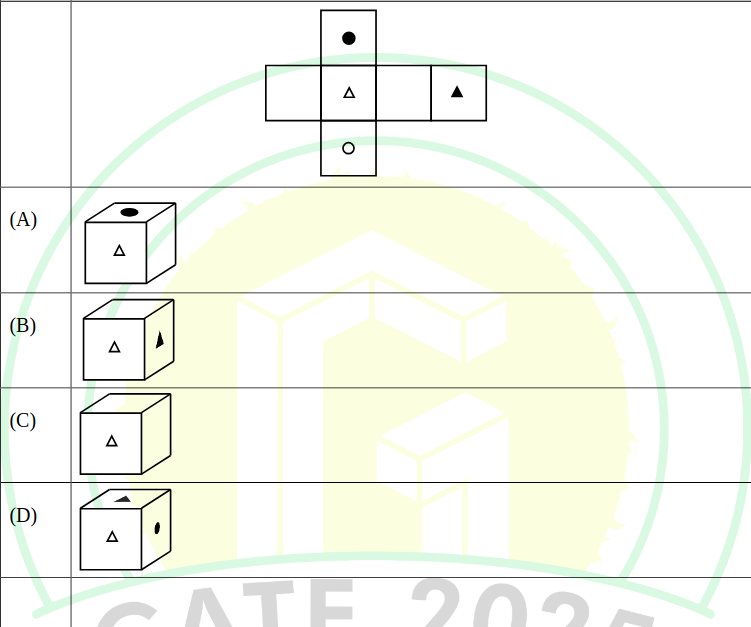
\includegraphics[width=0.7\columnwidth]{figs/Q.4.png} 
    \caption\centering{FIGURE}
    \label{fig:placeholder}
\end{figure}


\item Let $p_{1}$ and $p_{2}$ denote two arbitrary prime numbers. Which one of the following statements is correct for all values of $p_{1}$ and $p_{2}$? \hfill{\brak{\text{GATE MT 2025}}}
\begin{multicols}{2}
\begin{enumerate}
\item $p_{1}+p_{2}$ is not a prime number.
\item $p_{1}p_{2}$ is not a prime number.
\item $p_{1}+p_{2}+1$ is a prime number.
\item $p_{1}p_{2}+1$ is a prime number.
\end{enumerate}
\end{multicols}
\end{enumerate}

\subsection*{Q.6 - Q.10 Carry TWO marks Each}
\begin{enumerate}[resume]
\item Based only on the conversation below, identify the logically correct inference: \hfill{\brak{\text{GATE MT 2025}}} \\
"Even if I had known that you were in the hospital, I would not have gone there to see you", Ramya told Josephine.
\begin{enumerate}
    \item Ramya knew that Josephine was in the hospital.
    \item Ramya did not know that Josephine was in the hospital.
    \item Ramya and Josephine were once close friends; but now, they are not.
    \item Josephine was in the hospital due to an injury to her leg.
\end{enumerate}

\item If IMAGE and FIELD are coded as FHBNJ and EMFJG respectively then, which one among the given options is the most appropriate code for BEACH? \hfill{\brak{\text{GATE MT 2025}}}
\begin{multicols}{4}
\begin{enumerate}
\item CEADP
\item IDBFC
\item JGIBC
\item IBCEC
\end{enumerate}
\end{multicols}

\item Which one of the following options is correct for the given data in the table? \hfill{\brak{\text{GATE MT 2025}}}
\begin{center}
\begin{tabular}{|c|c|c|c|}
\hline
\textbf{Iteration (i)} & \textbf{Input (I)} & \textbf{Output (X)} & \textbf{Output (Y)} \\
\hline
0 & 20 & 20 & 20 \\
\hline
1 & -4 & 16 & -80 \\
\hline
2 & 10 & 26 & -800 \\
\hline
3 & 15 & 41 & -12000 \\
\hline
\end{tabular}
\end{center}
\begin{enumerate}
\item $X(i)=X(i-1)+I(i)$; $Y(i)=Y(i-1)I(i)$; $i>0$
\item $X(i)=X(i-1)I(i)$; $Y(i)=Y(i-1)+I(i)$; $i>0$
\item $X(i)=X(i-1)I(i)$; $Y(i)=Y(i-1)I(i)$; $i>0$
\item $X(i)=X(i-1)+I(i)$; $Y(i)=Y(i-1)I(i-1)$; $i>0$
\end{enumerate}

\item In the given figure, PQRS is a square of side 2 cm and PLMN is a rectangle. The corner L of the rectangle is on the side QR. Side MN of the rectangle passes through the corner S of the square. \hfill{\brak{\text{GATE MT 2025}}} \\
What is the area (in $cm^2$) of the rectangle PLMN? \\
Note: The figure shown is representative.
\begin{figure}[H]
    \centering
    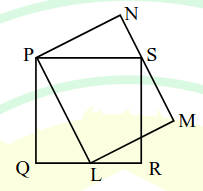
\includegraphics[width=0.2\columnwidth]{figs/Q.9.png}
    \caption\centering{FIGURE}
    \label{fig.placeholder}
\end{figure}
\begin{multicols}{4}
\begin{enumerate}
\item $2\sqrt{2}$
\item 2
\item 8
\item 4
\end{enumerate}
\end{multicols}

\item The diagram below shows a river system consisting of 7 segments, marked P, Q, R, S, T, U, and V. It splits the land into 5 zones, marked Z1, Z2, Z3, Z4, and Z5. We need to connect these zones using the least number of bridges. Out of the following options, which one is correct? \hfill{\brak{\text{GATE MT 2025}}} \\
Note: The figure shown is representative.
\begin{figure}[H]
    \centering
    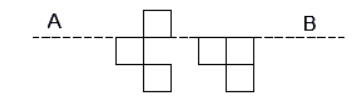
\includegraphics[width=0.5\columnwidth]{figs/Q.10.png}
    \caption\centering{RIVER SYSTEM}
    \label{fig.placeholder}
\end{figure}
\begin{enumerate}
\item Bridges on P, Q, and T
\item Bridges on P, Q, S, and T
\item Bridges on Q, R, T, and V
\item Bridges on P, Q, S, U, and V
\end{enumerate}
\end{enumerate}

\section*{Metallurgical Engineering}
\subsection*{Q.11 - Q.35 Carry ONE mark Each}
\begin{enumerate}[resume]
\item Which one of the following matrices has eigenvalues 1 and 6? \hfill{\brak{\text{GATE MT 2025}}}
\begin{multicols}{2}
\begin{enumerate}
\item $\myvec {5 & -2 \\ -2 & 2}$
\item $\myvec{3 & -1 \\ -2 & 2 }$
\item $\myvec{3 & -1 \\ -1 & 2}$
\item $\myvec{2 & -1 \\ -1 & 3}$
\end{enumerate}
\end{multicols}

\item For an isobaric process, the heat transferred is equal to the change in \underline{\hspace{2cm}} of the system. \hfill{\brak{\text{GATE MT 2025}}}
\begin{multicols}{2}
\begin{enumerate}
\item enthalpy
\item entropy
\item Helmholtz free energy
\item Gibbs free energy
\end{enumerate}
\end{multicols}

\item Match each crystal defect in Column I with the corresponding type in Column II. \hfill{\brak{\text{GATE MT 2025}}}
\begin{center}
\begin{tabular}{ll}
\textbf{Column I} & \textbf{Column II} \\
P. Edge dislocation & 1. Zero-dimensional defect \\
Q. Stacking fault & 2. One-dimensional defect \\
R. Frenkel defect & 3. Two-dimensional defect \\
S. Porosity & 4. Three-dimensional defect \\
\end{tabular}
\end{center}
\begin{enumerate}
\item P – 3, Q – 4, R – 2, S – 1  
\item P – 3, Q – 4, R – 1, S – 2  
\item P – 2, Q – 3, R – 1, S – 4
\item P – 2, Q – 4, R – 3, S – 1
\end{enumerate}

\item At high temperatures, which one of the following empirical expressions correctly describes the variation of dynamic viscosity $\mu$ of a Newtonian liquid with absolute temperature $T$? \hfill{\brak{\text{GATE MT 2025}}} \\
Given: $A$ and $B$ are positive constants.
\begin{multicols}{2}
\begin{enumerate}
\item $\mu = A + BT$
\item $\mu = A \exp(-BT)$
\item $\mu = A \exp(B/T)$ 
\item $\mu = A \exp(BT)$
\end{enumerate}
\end{multicols}

\item Which one of the following is an intensive property? \hfill{\brak{\text{GATE MT 2025}}}
\begin{multicols}{2}
\begin{enumerate}
\item Chemical potential
\item Volume
\item Mass
\item Entropy
\end{enumerate}
\end{multicols}

\item Hot metal from a blast furnace is treated with mill scale prior to oxygen steelmaking for \underline{\hspace{2cm}} \hfill{\brak{\text{GATE MT 2025}}}
\begin{multicols}{2}
\begin{enumerate}
\item dephosphorization
\item decarburization
\item desulphurization
\item desiliconization
\end{enumerate}
\end{multicols}

\item In optical microscopy, which one of the following combinations of wavelength ($\lambda$) and numerical aperture (NA) provides the best spatial resolution? \hfill{\brak{\text{GATE MT 2025}}}
\begin{multicols}{2}
\begin{enumerate}
\item $\lambda = 400$ nm and NA = 1.0
\item $\lambda = 600$ nm and NA = 1.2
\item $\lambda = 400$ nm and NA = 1.2
\item $\lambda = 600$ nm and NA = 1.0
\end{enumerate}
\end{multicols}

\item The coordination number for an octahedral site in pure copper is \underline{\hspace{2cm}}. \hfill{\brak{\text{GATE MT 2025}}}
\begin{multicols}{4}
\begin{enumerate}
\item 4
\item 6
\item 8
\item 12
\end{enumerate}
\end{multicols}

\item Consider the following gas-phase reaction: \hfill{\brak{\text{GATE MT 2025}}} \\
\begin{align}
 2SO_2 + O_2 \rightleftharpoons 2SO_3 \
\end{align}
If the enthalpy of reaction is negative, which one of the following conditions promotes a higher equilibrium concentration of $SO_3$?
\begin{enumerate}
\item Higher pressure and higher temperature
\item Higher pressure and lower temperature
\item Lower pressure and higher temperature
\item Lower pressure and lower temperature
\end{enumerate}

\item Which one of the following slag components is responsible for the oxidizing power of steelmaking slags? \hfill{\brak{\text{GATE MT 2025}}}
\begin{multicols}{4}
\begin{enumerate}
\item $SiO_2$
\item $CaO$
\item $MgO$
\item $FeO$
\end{enumerate}
\end{multicols}

\item Two randomly oriented polycrystalline copper samples with average grain sizes of $10 \micro m$ (Sample A) and $100 \micro m$ (Sample B) were tested at room temperature. \hfill{\brak{\text{GATE MT 2025}}} \\
Given: \\
$E_A$ = Young’s modulus of Sample A \\
$E_B$ = Young’s modulus of Sample B \\
$YS_A$ = Yield strength of Sample A \\
$YS_B$ = Yield strength of Sample B \\
Which one of the following statements is CORRECT?
\begin{enumerate}
\item $E_A > E_B$ and $YS_A > YS_B$
\item $E_A = E_B$ and $YS_A < YS_B$
\item $E_A > E_B$ and $YS_A = YS_B$
\item $E_A = E_B$ and $YS_A > YS_B$
\end{enumerate}

\item In metal casting, which one of the following gating ratios (sprue-runner-gate area ratio) represents a non-pressurized gating system? \hfill{\brak{\text{GATE MT 2025}}}
\begin{multicols}{4}
\begin{enumerate}
\item 1 : 2 : 3
\item 3 : 2 : 1
\item 4 : 3 : 1
\item 5 : 4 : 1
\end{enumerate}
\end{multicols}

\item In the Fe-C system, the invariant reaction Liquid + $\delta \rightleftharpoons \gamma$ takes place at 1493 \degree C. This type of reaction is called \underline{\hspace{2cm}}. \hfill{\brak{\text{GATE MT 2025}}}
\begin{multicols}{4}
\begin{enumerate}
\item eutectic
\item eutectoid
\item peritectic
\item monotectic
\end{enumerate}
\end{multicols}

\item Match the following elements in Column I with their respective ores in Column II. \hfill{\brak{\text{GATE MT 2025}}}
\begin{center}
\begin{tabular}{ll}
\textbf{Column I} & \textbf{Column II} \\
P. Al & 1. Rutile \\
Q. Fe & 2. Hematite \\
R. Ti & 3. Chalcopyrite \\
S. Cu & 4. Bauxite \\
\end{tabular}
\end{center}
\begin{enumerate}
\item P – 4, Q – 2, R – 3, S – 1
\item P – 2, Q – 4, R – 1, S – 3
\item P – 3, Q – 1, R – 4, S – 2
\item P – 4, Q – 2, R – 1, S – 3
\end{enumerate}

\item Which of the following functions is/are expandable using Maclaurin series? \hfill{\brak{\text{GATE MT 2025}}}
\begin{multicols}{4}
\begin{enumerate}
\item $\ln(1 + z)$
\item $\ln z$
\item $\frac{1}{z^2}$
\item $\exp(z)$
\end{enumerate}
\end{multicols}

\item With reference to edge and screw dislocations, which of the following statements is/are CORRECT? \hfill{\brak{\text{GATE MT 2025}}}
\begin{enumerate}
\item Both edge and screw dislocations can leave the slip plane by climb.
\item Burgers vector of a screw dislocation is parallel to its line vector.
\item Both edge and screw dislocations can leave the slip plane by cross-slip.
\item Strain energy per unit length of an edge dislocation is higher than that of a screw dislocation.
\end{enumerate}

\item Which of the following conditions is/are favorable for producing low-silicon hot metal in blast furnace ironmaking? \hfill{\brak{\text{GATE MT 2025}}}
\begin{enumerate}
\item Reduced raceway adiabatic flame temperature
\item Oxygen-enriched blast
\item Lime injection through tuyeres
\item Increased hearth temperature
\end{enumerate}

\item Which of the following statements is/are CORRECT with respect to the initial stage of GP zone formation in a precipitation hardenable $Al - 4.5 wt.\%$ Cu alloy? \hfill{\brak{\text{GATE MT 2025}}}
\begin{enumerate}
\item GP zones are Cu-rich clusters.
\item GP zones are \ce{CuAl2} precipitates.
\item GP zones are incoherent with the matrix.
\item GP zones are coherent with the matrix.
\end{enumerate}

\item Which of the following techniques can be used to detect an internal defect in a metal casting? \hfill{\brak{\text{GATE MT 2025}}}
\begin{enumerate}
\item Ultrasonic inspection
\item Liquid (or dye) penetrant inspection
\item Gamma-ray radiography
\item X-ray radiography
\end{enumerate}

\item Standard Gibbs free energies of formation of some solid oxides per mole of $O_2$ at 1000 K are given below. \hfill{\brak{\text{GATE MT 2025}}} \\
$SiO_2: -728 kJ$, $TiO_2: -737 kJ$, $VO: -712 kJ$, $MnO: -624 kJ$ \\
Regarding thermodynamic feasibility of oxide reduction, which of the following statements is/are CORRECT under standard conditions at 1000 K?
\begin{enumerate}
\item Si can reduce $TiO_2$.
\item Mn can reduce $VO$.
\item Ti can reduce $MnO$.
\item V can reduce $SiO_2$.
\end{enumerate}

\item Consider a fully developed, steady, one-dimensional, laminar flow of a Newtonian liquid through a pipe. The maximum velocity in the pipe is proportional to which of the following quantities? \hfill{\brak{\text{GATE MT 2025}}} \\
Given: $\Delta P$ is the difference between the outlet and inlet pressure, $\mu$ is the dynamic viscosity of the liquid, and $R$ and $L$ are radius and length of the pipe, respectively.
\begin{multicols}{4}
\begin{enumerate}
\item $\Delta P$
\item $1/R^2$
\item $1/\mu$
\item $1/L$
\end{enumerate}
\end{multicols}

\item The hydrostatic stress for the stress tensor provided below is \underline{\hspace{2cm}} MPa (in integer). \hfill{\brak{\text{GATE MT 2025}}}
\begin{align}
    \myvec{
150 & 0 & 0 \\
0 & -100 & 100 \\
0 & 100 & 250}
\end{align}

\item For an application where the Reynolds number is to be kept constant, a liquid with a density of 1 g cm$^{-3}$ and viscosity 0.01 Poise results in a characteristic speed of 1 cm s$^{-1}$. If this liquid is replaced by another with a density of 1.25 g cm$^{-3}$ and viscosity of 0.015 Poise, the characteristic velocity will be \underline{\hspace{2cm}} cm s$^{-1}$ (rounded off to one decimal place). \hfill{\brak{\text{GATE MT 2025}}} \\
Assume the characteristic length of the flow to be the same in both cases.

\item Consider the gas phase reaction: \hfill{\brak{\text{GATE MT 2025}}} 
\begin{align}
CO + \frac{1}{2}O_2 \rightleftharpoons CO_2
\end{align}
At equilibrium for a particular temperature, the partial pressures of CO, \ce{O2}, and \ce{CO2} are found to be $10^{-6}$ atm, $10^{-6}$ atm, and 16 atm, respectively. The equilibrium constant for the reaction is \underline{\hspace{2cm}} $\times 10^{10}$ (rounded off to one decimal place).

\item A linear regression model was fitted to a set of ($x, y$) data. The total sum of squares and sum of squares of error are 1200 and 120, respectively. The coefficient of determination ($R^2$) of the fit is \underline{\hspace{2cm}} (rounded off to one decimal place). \hfill{\brak{\text{GATE MT 2025}}}
\end{enumerate}

\subsection*{Q.36 - Q.65 Carry TWO marks Each}
\begin{enumerate}[resume]
\item For two continuous functions $M(x, y)$ and $N(x, y)$, the relation $M dx + N dy = 0$ describes an exact differential equation if \hfill{\brak{\text{GATE MT 2025}}}
\begin{multicols}{4}
\begin{enumerate}
\item $\frac{\partial M}{\partial x} = \frac{\partial N}{\partial y}$
\item $\frac{\partial M}{\partial x} = -\frac{\partial N}{\partial y}$
\item $\frac{\partial M}{\partial y} = \frac{\partial N}{\partial x}$
\item $\frac{\partial M}{\partial y} = -\frac{\partial N}{\partial x}$
\end{enumerate}
\end{multicols}

\item Consider the phase diagram of a one component system given below. \hfill{\brak{\text{GATE MT 2025}}} \\
$V_\alpha$, $V_\beta$, and $V_{\text{Liquid}}$ are the molar volumes of $\alpha$, $\beta$, and liquid phases, respectively. Which one of the following statements is TRUE? \\
Given: The change in molar enthalpies, $\Delta H_{\alpha \to \beta}$ and $\Delta H_{\beta \to \text{Liquid}}$, are positive.
\begin{figure}[H]
    \centering
    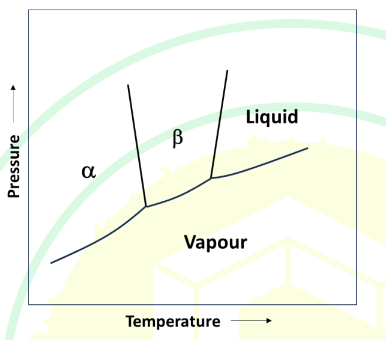
\includegraphics[width=0.3\columnwidth]{figs/Q.37.png}
    \caption\centering{PHASE DIAGRAM}
    \label{fig.placeholder}
\end{figure}
\begin{enumerate}
\item $V_\alpha < V_\beta$ and $V_\beta < V_{\text{Liquid}}$
\item $V_\alpha > V_\beta$ and $V_\beta < V_{\text{Liquid}}$
\item $V_\alpha < V_\beta$ and $V_\beta > V_{\text{Liquid}}$
\item $V_\alpha > V_\beta$ and $V_\beta > V_{\text{Liquid}}$
\end{enumerate}

\item Match the steel plant related processes in Column I with the associated information in Column II. \hfill{\brak{\text{GATE MT 2025}}}
\begin{center}
\begin{tabular}{ll}
\textbf{Column I} & \textbf{Column II} \\
P. Corex & 1. Melter-gasifier \\
Q. Electric Arc Furnace & 2. Natural gas reformer \\
R. Midrex & 3. Electromagnetic stirrer \\
S. Continuous Casting & 4. Hot heel \\
\end{tabular}
\end{center}
\begin{enumerate}
\item P – 1, Q – 4, R – 2, S – 3
\item P – 1, Q – 4, R – 3, S – 2
\item P – 2, Q – 4, R – 1, S – 3
\item P – 1, Q – 3, R – 2, S – 4
\end{enumerate}

\item Radiative heat flux $\dot{q}$ at a hot surface at a temperature $T_s$ can be expressed as \hfill{\brak{\text{GATE MT 2025}}}
\begin{align}
\dot{q} = A f(T_s, T_\infty) (T_s - T_\infty) 
\end{align}
where $A$ is a constant and $T_\infty$ is the temperature of the surroundings (temperatures are expressed in K). The function $f(T_s, T_\infty)$ is given by \underline{\hspace{2cm}}.
\begin{enumerate}
\item $(T_s + T_\infty)^2(T_s - T_\infty)$
\item $(T_s^2 + T_\infty^2)(T_s + T_\infty)$
\item $(T_s^2 - T_\infty^2) (T_s + T_\infty)$
\item $(T_s - T_\infty)^2(T_s + T_\infty)$
\end{enumerate}

\item Match the phenomena in Column I with the typical observations in Column II. \hfill{\brak{\text{GATE MT 2025}}}
\begin{center}
\begin{tabular}{ll}
\textbf{Column I} & \textbf{Column II} \\
P. Dynamic strain aging & 1. Grain boundary sliding \\
Q. Recrystallization & 2. Decrease in yield stress with a \\ & reversal of loading direction \\
R. Bauschinger effect & 3. Decrease in dislocation density \\
S. Superplasticity & 4. Serrations in stress-strain curve \\
\end{tabular}
\end{center}
\begin{enumerate}
\item P – 4, Q – 1, R – 2, S – 3 
\item P – 4, Q – 3, R – 2, S – 1 
\item P – 3, Q – 4, R – 2, S – 1 
\item P – 1, Q – 4, R – 2, S – 3
\end{enumerate}

\item Which one of the following matrices is orthogonal? \hfill{\brak{\text{GATE MT 2025}}}
\begin{multicols}{2}
\begin{enumerate}
\item $\begin{pmatrix} 1/2 & -\sqrt{3}/2 \\ -\sqrt{3}/2 & 1/2 \end{pmatrix}$
\item $\begin{pmatrix} 1/2 & -\sqrt{3}/2 \\ \sqrt{3}/2 & 1/2 \end{pmatrix}$
\item $\begin{pmatrix} 1/\sqrt{2} & -\sqrt{3}/2 \\ -\sqrt{3}/2 & 1/2 \end{pmatrix}$
\item $\begin{pmatrix} 1/\sqrt{2} & -\sqrt{3}/2 \\ \sqrt{3}/2 & -1/\sqrt{2} \end{pmatrix}$
\end{enumerate}
\end{multicols}

\item Match the casting defects in Column I with the characteristic features in Column II. \hfill{\brak{\text{GATE MT 2025}}}
\begin{center}
\begin{tabular}{ll}
\textbf{Column I} & \textbf{Column II} \\
P. Misrun & 1. Penetration of liquid metal behind \\ & surface layer of sand moulds \\
Q. Expansion scab & 2. Metal solidifies prematurely in the \\ & mould and some sections of the \\ & casting are not filled \\
R. Pin holes & 3. Cracking because of restraint to \\ & contraction in certain areas of the \\ & casting during solidification and \\ & cooling to room temperature \\
S. Hot tearing & 4. Evolution of gases during \\ & solidification resulting in porosity \\
\end{tabular}
\end{center}
\begin{enumerate}
\item P – 2, Q – 4, R – 3, S – 1 
\item P – 1, Q – 3, R – 2, S – 4 
\item P – 1, Q – 2, R – 4, S – 3
\item P – 2, Q – 1, R – 4, S – 3
\end{enumerate}

\item The following are the activation energies for diffusion of carbon and iron at 773 K in polycrystalline BCC iron: \hfill{\brak{\text{GATE MT 2025}}} \\
P = Activation energy for diffusion of carbon in BCC iron through the lattice \\
Q = Activation energy for diffusion of iron in BCC iron through the lattice \\
R = Activation energy for diffusion of iron in BCC iron along the grain boundary \\
Which one of the following statements is CORRECT?
\begin{multicols}{4}
\begin{enumerate}
\item $R < P < Q$
\item $R < Q < P$
\item $Q < P < R$
\item $P < R < Q$
\end{enumerate}
\end{multicols}

\item Front tension is applied during cold rolling of a thin metal sheet. Which of the following statements is/are TRUE? \hfill{\brak{\text{GATE MT 2025}}}
\begin{enumerate}
\item The neutral point shifts towards the roll entrance.
\item The rolling load is decreased.
\item The neutral point shifts towards the roll exit.
\item The rolling load is increased.
\end{enumerate}

\item Which of the following statements is/are CORRECT when Ni is added as an alloying element to a low alloy steel? \hfill{\brak{\text{GATE MT 2025}}}
\begin{enumerate}
\item Hardenability is increased AND the Ms temperature is lowered.
\item Hardenability is decreased AND the Ms temperature is lowered.
\item Hardenability is increased AND the Ms temperature is raised.
\item Hardenability is decreased AND the Ms temperature is raised.
\end{enumerate}

\item Which of the following statements is/are CORRECT with respect to fusion welding and solid-state welding of metals and alloys? \hfill{\brak{\text{GATE MT 2025}}}
\begin{enumerate}
\item Thermomechanically affected zone is found in the fusion welding of pure metals.
\item Partially melted zone is NOT found in the fusion welding of pure metal.
\item Diffusion bonding is one type of solid-state welding process.
\item Partially melted zone is found in the fusion welding of alloys with a large freezing range.
\end{enumerate}

\item Which of the following welding processes does NOT / do NOT utilize consumable electrode? \hfill{\brak{\text{GATE MT 2025}}}
\begin{multicols}{2}
\begin{enumerate}
\item Plasma arc welding
\item Gas metal arc welding
\item Shielded metal arc welding
\item Electron beam welding
\end{enumerate}
\end{multicols}

\item For a two-dimensional field described by $T(x, y) = \frac{1}{3}xy(x + y)$, the magnitude of its gradient at the point (1,1) is \underline{\hspace{2cm}} (rounded off to two decimal places). \hfill{\brak{\text{GATE MT 2025}}}

\item X-ray diffraction using a monochromatic radiation of wavelength 0.154 nm is performed on powder samples of metal A (with FCC crystal structure) and metal B (with BCC crystal structure). If the first peak in both the cases occurs at a Bragg angle $\theta = 20\degree$, then the value of $\frac{\text{lattice parameter of metal A}}{\text{lattice parameter of metal B}}$ = \underline{\hspace{2cm}} (rounded off to two decimal places). \hfill{\brak{\text{GATE MT 2025}}}

\item The excess molar Gibbs free energy of a solution of element A and B at 1000 K is given by $G^{XS} = -3000 X_A X_B$ J mol$^{-1}$, where $X_A$ and $X_B$ are mole fractions of A and B, respectively. The activity of B in a solution of A and B containing 40 mol\% of B at 1000 K is \underline{\hspace{2cm}} (rounded off to two decimal places). \hfill{\brak{\text{GATE MT 2025}}} \\
Given: Ideal gas constant R = 8.314 J mol$^{-1}$ K$^{-1}$.

\item Molten steel at 1900 K having dissolved hydrogen needs to be vacuum degassed. The equilibrium partial pressure of hydrogen to be maintained to achieve 1 ppm (mass basis) of dissolved hydrogen is \underline{\hspace{2cm}} Torr (rounded off to two decimal places). \hfill{\brak{\text{GATE MT 2025}}} \\
Given: For the hydrogen dissolution reaction in molten steel (½ \ce{H2(g)} = [H]), the equilibrium constant (expressed in terms of ppm of dissolved H) is: \\
$\log_{10} K_{eq} = -\frac{1900}{T} + 2.4$ \\
1 atm = 760 Torr

\item The value of $\lim_{x\to0} \frac{6(x-\sin x)}{x^3}$ is \underline{\hspace{2cm}} (in integer). \hfill{\brak{\text{GATE MT 2025}}}

\item Consider the following reactions and their standard Gibbs free energies (in J): \hfill{\brak{\text{GATE MT 2025}}} 
\begin{align}
Fe(s) + \frac{1}{2}O_2(g) \rightleftharpoons FeO(s)\; \;\Delta G\degree = -264900 + 65T\\
2 H_2(g) + O_2(g) \rightleftharpoons 2 H_2O(g) \;\;\Delta G\degree = -492900 + 109T
\end{align}
Assuming Fe and FeO to be pure and no solubility of gases in the solids, the value of $\frac{p_{H_2O}}{p_{H_2}}$ required to reduce solid $FeO$ to solid Fe at 1000 K is \underline{\hspace{2cm}} (rounded off to two decimal places). \\
Given: Ideal gas constant R = 8.314 J mol$^{-1}$ K$^{-1}$.

\item The diameter of spherical galena particles that have the same settling velocity as spherical quartz particles of diameter $25\micro m$ (both settling in water) is \underline{\hspace{2cm}} $\micro m$ (rounded off to one decimal place). \hfill{\brak{\text{GATE MT 2025}}} \\
Assume Stokes law of settling to be valid. \\
Given: Density of galena = 7400 kg m$^{-3}$, density of quartz = 2600 kg m$^{-3}$, density of water = 1000 kg m$^{-3}$.

\item Consider the following cell reaction: \hfill{\brak{\text{GATE MT 2025}}} 
\begin{align}
Mg + Cd^{2+} \rightleftharpoons Mg^{2+} + Cd
\end{align}
The standard Gibbs free energy change for the reaction is \underline{\hspace{2cm}} kJ (rounded off to an integer). \\
Given: Standard oxidation potentials for the reactions with respect to standard hydrogen electrode are: \\
$Mg \rightleftharpoons Mg^{2+} + 2e^-\;\;E\degree = 2.37$ V \\
$Cd \rightleftharpoons Cd^{2+} + 2e^- \;\; E\degree = 0.403$ V \\
Faraday’s constant = 96500 C mol$^{-1}$.

\item Copper is being electrodeposited from a $CuSO_4$ bath onto a stainless steel cathode of total surface area of 2 m$^2$ in an electrolytic cell operated at a current density of 200 A m$^{-2}$ with a current efficiency of $90\%$. The mass of copper deposited in 24 h is \underline{\hspace{2cm}} kg (rounded off to two decimal places). \hfill{\brak{\text{GATE MT 2025}}} \\
Given: Faraday’s constant = 96500 C mol$^{-1}$, atomic mass of copper = 63.5 g mol$^{-1}$.

\item An intrinsic semiconductor has conductivity of 100 $\Omega^{-1}$ m$^{-1}$ at 300 K and 300 $\Omega^{-1}$ m$^{-1}$ at 500 K. The band gap of the semiconductor is \underline{\hspace{2cm}} eV (rounded off to two decimal places). \hfill{\brak{\text{GATE MT 2025}}} \\
Given: Boltzmann constant $k_B = 8.6 \times 10^{-5}$ eV K$^{-1}$.

\item For a component fabricated from an alloy A with plane strain fracture toughness, $K_{IC}$ = 50 MPa m$^{1/2}$, fracture was observed to take place at a crack length of 0.4 mm at a tensile service stress of $\sigma$. If the same component is instead fabricated from alloy B with $K_{IC}$ = 75 MPa m$^{1/2}$, the crack length at which a similar crack geometry will result in fracture (under identical tensile service stress of $\sigma$) is \underline{\hspace{2cm}} mm (rounded off to one decimal place). \hfill{\brak{\text{GATE MT 2025}}}

\item Temperatures at two sides of a 0.4 m thick copper plate are 1000 and $500 \degree C$. Assuming steady state, one-dimensional conductive heat transfer through the wall and ignoring end-effects, the magnitude of the heat flux through the wall is \underline{\hspace{2cm}} $\times 10^5$ W m$^{-2}$ (in integer). \hfill{\brak{\text{GATE MT 2025}}} \\
Given: Thermal conductivity of copper is 400 W m$^{-1}$ K$^{-1}$.

\item In polycrystalline Ni, Nabarro-Herring diffusion creep was found to be the rate controlling creep mechanism at a certain temperature. At that temperature, if the steady state strain rate is $10^{-8}$ s$^{-1}$ at a stress of 10 MPa, the steady state strain rate of $10^{-9}$ s$^{-1}$ will be obtained at a stress value of \underline{\hspace{2cm}} MPa (in integer). \hfill{\brak{\text{GATE MT 2025}}} \\
Assume that the same creep mechanism is rate controlling during the creep deformation.

\item A single crystal BCC metal with a lattice parameter $a = 0.4$ nm is subjected to deformation at a shear strain rate of 0.001 s$^{-1}$. If the average mobile dislocation density in the single crystal is $10^{10}$ m$^{-2}$, the average dislocation velocity is \underline{\hspace{2cm}} $\times 10^{-3}$ m s$^{-1}$ (rounded off to two decimal places). \hfill{\brak{\text{GATE MT 2025}}} \\
Given: Burgers vector $\mathbf{b} = \frac{a}{2}\langle111\rangle$.

\item A cylindrical specimen is subjected to plastic deformation in tension up to a uniform elongation of 10\%. The final cross-sectional area of the gage section is found to be 20 mm$^2$. The initial cross-sectional area of the gage section is \underline{\hspace{2cm}} mm$^2$ (rounded off to an integer). \hfill{\brak{\text{GATE MT 2025}}}

\item The reaction represented by $A \longrightarrow B$ follows first order kinetics. At a given temperature, $20\%$ of the reaction is completed in 223 s. The time taken to complete $50\%$ of the reaction at the same temperature is \underline{\hspace{2cm}} s (rounded off to the nearest integer). \hfill{\brak{\text{GATE MT 2025}}}

\item A cylindrical Al alloy billet of 300 mm diameter is hot extruded to produce a cylindrical rod of 75 mm diameter at a constant true strain rate ($\dot{\epsilon}$) of 10 s$^{-1}$. The flow stress ($\sigma$) of the alloy at the extrusion temperature is given by $\sigma = 10 (\dot{\epsilon})^{0.3}$ MPa. Assume the alloy is perfectly plastic and there is no temperature rise during the extrusion process. The ideal plastic work of deformation per unit volume is \underline{\hspace{2cm}} $\times 10^6$ J m$^{-3}$ (rounded off to one decimal place). \hfill{\brak{\text{GATE MT 2025}}}

\item Two consecutive estimates of the root of a function $f(x)$ obtained using the Newton-Raphson method are $x_i = 8.5$ and $x_{i+1} = 13.5$, and the value of the function at $x_i$ is 15. The numerical value of first derivative of the function evaluated at $x_i$ is \underline{\hspace{2cm}} (in integer). \hfill{\brak{\text{GATE MT 2025}}}

\end{enumerate}

\section*{*END OF THE QUESTION PAPER*}
 
\end{document}